\documentclass[letterpaper]{article}

\usepackage[margin=2.2cm]{geometry}
\usepackage[spanish,es-nodecimaldot]{babel}
\usepackage[utf8]{inputenc}
\usepackage[T1]{fontenc}
\usepackage{graphicx}
\usepackage{grffile}
\usepackage{longtable}
\usepackage{wrapfig}
\usepackage{rotating}
\usepackage[normalem]{ulem}
\usepackage{amsmath}
\usepackage{textcomp}
\usepackage{amssymb}
\usepackage{capt-of}
\usepackage{hyperref}
\usepackage{minted}
\usepackage{subfiles}
\usepackage[acronym, toc]{glossaries}

\usepackage{fancyhdr}
\usepackage{graphicx}
\usepackage{xcolor}
\usepackage{multicol}

\usepackage{grffile}
\usepackage{longtable}
\usepackage{wrapfig}
\usepackage{rotating}
\usepackage[normalem]{ulem}
\usepackage{amsmath}
\usepackage{textcomp}
\usepackage{amssymb}
\usepackage{capt-of}
\usepackage{hyperref}

\definecolor{LightGray}{gray}{0.9}
\definecolor{DarkGray}{gray}{0.1}
\definecolor{Base03}{HTML}{f8f8f8}

\usemintedstyle{emacs}



\renewcommand{\listingscaption}{Script}
\renewcommand\listoflistingscaption{Índice de \listingscaption\@'s}
\setminted[bash]{frame=lines,framesep=2mm,baselinestretch=1.2,fontsize=\scriptsize,breaklines=true,bgcolor=Base03}
\setminted[bat]{frame=lines,framesep=2mm,baselinestretch=1.2,fontsize=\scriptsize,breaklines=true,bgcolor=Base03}
\setminted[linux-config]{frame=lines,framesep=2mm,baselinestretch=1.2,fontsize=\scriptsize,breaklines=true,bgcolor=Base03}
\setminted[shell-session]{frame=lines,framesep=2mm,baselinestretch=1.2,fontsize=\scriptsize,breaklines=true,bgcolor=Base03}
\graphicspath{{./img_common}{../images}}
% \pagestyle{fancy}
% \fancyfoot[R]{\thepage}
% \fancyfoot[C]{
\includegraphics[width=0.1\textwidth]{inge_logo}}
% \fancyhead[L]{\leftmark}
% \fancyhead[R]{\rightmark}

\hypersetup{
 pdfauthor={Gonzalez Gonzalez Claudio, Mansur Jiménez Arturo, Romero Andrade Cristian, Romero Andrade Vicente},
 pdftitle={Proyecto SD},
 pdfkeywords={},
 pdfsubject={},
 pdfcreator={LuaTex},
 pdflang={Spanish}}

\title{Proyecto: Implementación de un servidor con sincronización usando NIS-SAMBA-Active Directory}

\author{
  \IEEEauthorblockN{Gonzalez Gonzalez Claudio,
  Mansur Jiménez Arturo,
    Romero Andrade Cristian,
    Romero Andrade Vicente}
  \IEEEauthorblockA{Sistemas Distribuidos\\
Facultad de Ingeniería\\
Universidad Nacional Autónoma de México\\
}}
\newcommand\indexspace{\par \vskip 15\p@ \@plus5\p@ \@minus3\p@\relax}
\usepackage{microtype}



\newglossaryentry{SAMBA}
{
  name=SAMBA,
  description={Es una implementación libre del protocolo de archivos
    compartidos de Microsoft Windows para sistemas de tipo UNIX}
}
\newglossaryentry{ldap}
{
  name=LDAP,
  description={El protocolo ligero de acceso a directorios hace referencia a un
    protocolo a nivel de aplicación que permite el acceso a un servicio de
    directorio ordenado y distribuido para buscar diversa información en un
    entorno de red}
}

\newglossaryentry{kerberos}
{
  name=Kerberos,
  description={Es un protocolo de autenticación de redes de ordenador creado
    por el MIT que permite a dos ordenadores en una red insegura demostrar
    su identidad mutuamente de manera segura}
}

\newglossaryentry{nfs}
{
  name=NFS,
  description={Network File System es un
    protocolo de nivel de aplicación, según el Modelo OSI.~Es utilizado para
    sistemas de archivos distribuido en un entorno de red de computadoras de
    área local. Posibilita que distintos sistemas conectados a una misma red
    accedan a ficheros remotos}
}

\newglossaryentry{autofs}
{
  name=AutoFS,
  description={Es un servicio por parte del cliente que monta
    automáticamente el sistema de archivos adecuado.}
}

\newglossaryentry{fstab}
{
  name=fstab,
  description={Es un fichero que se encuentra comúnmente en
    sistemas Unix (en el directorio \texttt{/etc/}) como parte de la
    configuración del sistema. Lo más destacado de este fichero es la lista de
    discos y particiones disponibles. En ella se indica como montar cada
    dispositivo y qué configuración utilizar}
}

\newglossaryentry{systemd}
{
  name=systemd,
  description={Es un conjunto de demonios o daemons de
    administración de sistema, bibliotecas y herramientas diseñados como una
    plataforma de administración y configuración central para interactuar con
    el núcleo del Sistema operativo GNU/Linux.}
}






\newacronym{ntp}{NTP}{Network Time Protocol}
\newacronym{nfs}{NFS}{Network File System}
\newacronym{nis}{NIS}{Network Information Service}
\newacronym{smb}{SMB}{Server Message Block}

\makeglossaries{}

\begin{document}

\begin{titlepage}
  \centering{
    
\includegraphics[width=0.3\textwidth]{unam_logo}\vfill{}
    {\scshape{\Huge Facultad de Ingeniería\par{}}}\vspace{0.5cm}
    {\scshape{\Large Sistemas Distribuidos\par{}}}\vfill{}
    {\huge \textbf{Proyecto}}\vfill{}

    {\Large
      Alumnos
      \begin{itemize}
        \item Gonzalez Gonzalez Claudio
        \item Mansur Jiménez Arturo
        \item Romero Andrade Cristian
        \item Romero Andrade Vicente
      \end{itemize}
      % \textbf{Equipo  }

    }\vfill{}
    {\large Profesor: ING.~Guadalupe Lizeth Parrales Romay}\vfill{}
    
\includegraphics[width=0.1\textwidth]{inge_logo}
  }
\end{titlepage}


\addcontentsline{toc}{section}{Portada}
\tableofcontents
\addcontentsline{toc}{section}{Índice}


\newpage


\section{Introducción}\label{sec:introduccion}
En al presente se presenta la implementación de una distribución de información
a varías maquinas que estén conectadas a una red mediante el uso de distintos
protocolos de sincronización (implementado en la sección~\ref{sec:samba_addc})
y distribución de información.


\section{Arquitectura}\label{sec:arq}
\begin{figure}[h!]
  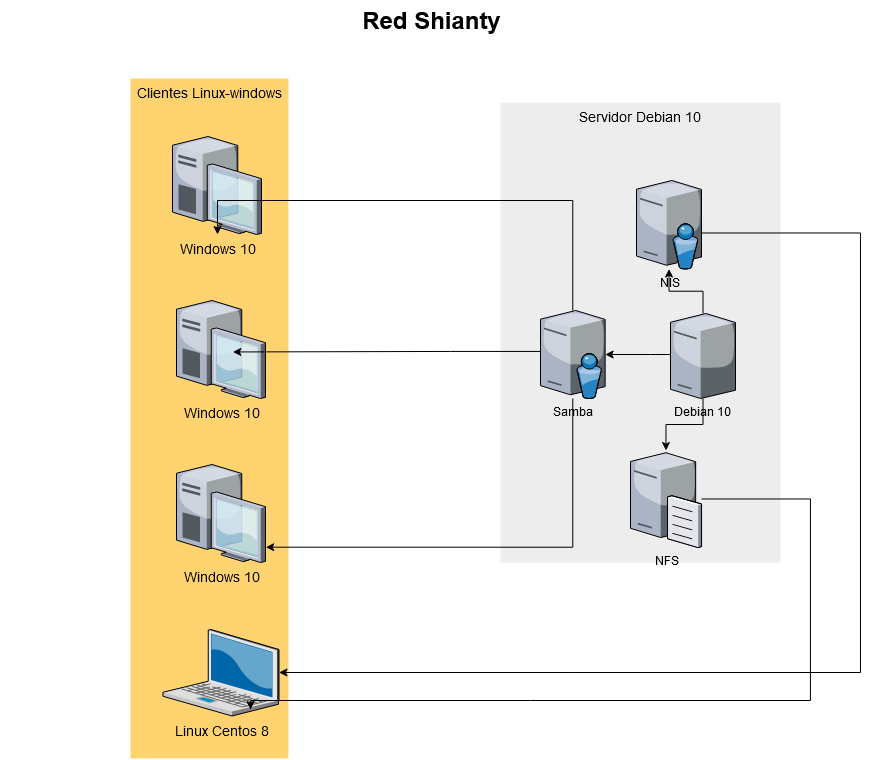
\includegraphics[width=0.9\textwidth]{arquitectura}
  \caption{Arquitectura de la red}\label{fig:arquitectura}
\end{figure}

\begin{figure}[h!]
  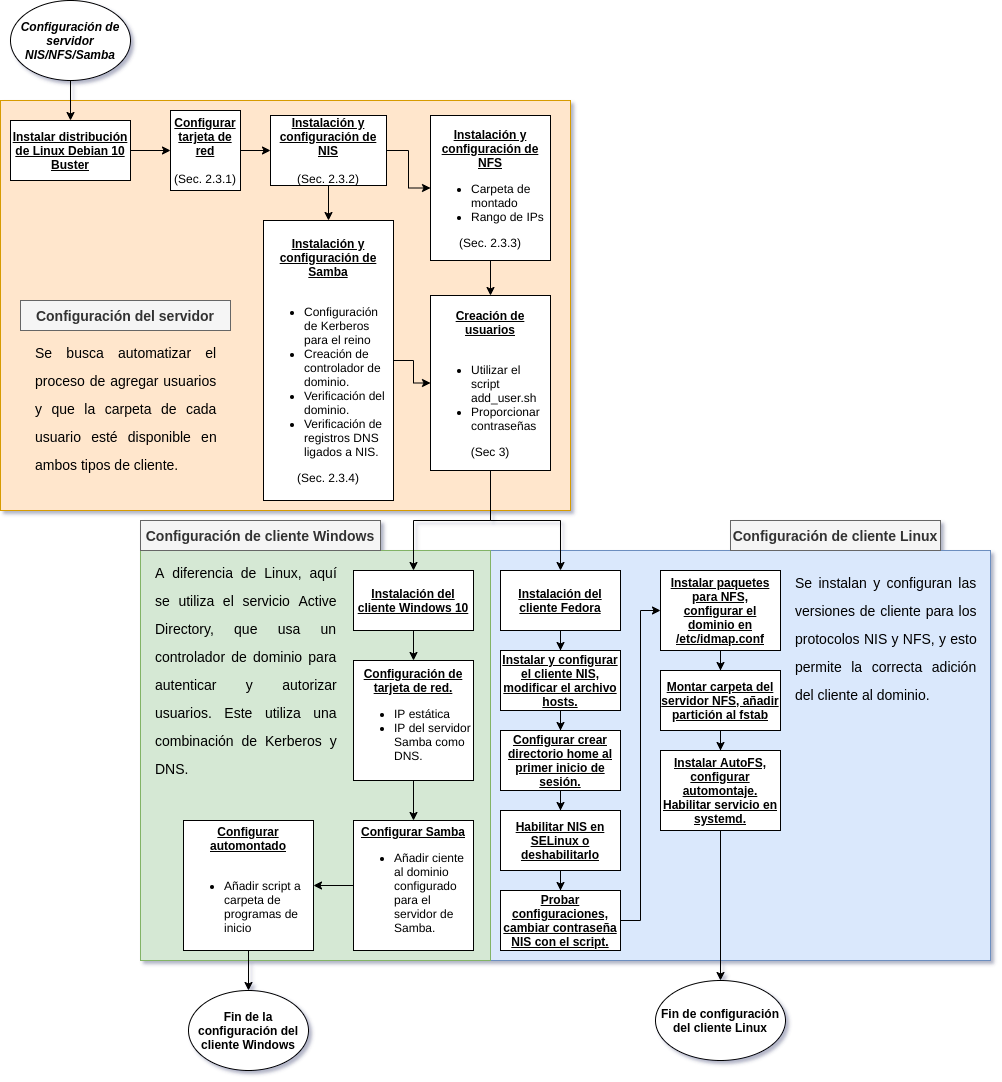
\includegraphics[width=0.9\textwidth]{Diagrama_Shianty}
  \caption{Diagrama cliente-servidor}\label{fig:dia_c_s}
\end{figure}



\section{Recursos}\label{sec:recursos}

\subfile{contenido/material_utilizado.tex}

\clearpage{}

\section{Creación de Usuarios}\label{sec:cusuarios}

\subfile{contenido/usuarios.tex}

\clearpage{}

\section{Clientes}\label{sec:clientes}

\subfile{contenido/cliente.tex}

\newpage

\addcontentsline{toc}{section}{Índice de figuras}
\listoffigures
\addcontentsline{toc}{section}{Índice de códigos}
\listoflistings{}
\newpage{}
\printglossary{}
\printglossary[type=\acronymtype]


\end{document}
